\documentclass[a4paper,12pt, twoside]{article}

\textwidth 17cm \textheight 25cm \evensidemargin 0cm
\oddsidemargin 0cm \topmargin -2cm
\parindent 0pt
%\parskip \bigskipamount

\usepackage{graphicx}
\usepackage[dutch]{babel}
\usepackage{amssymb,amsthm,amsmath}
%\usepackage{dot2texi}
\usepackage[utf8]{inputenc}
\usepackage{nopageno}
\usepackage{pdfpages}
\usepackage{enumerate}
\usepackage{caption}
\usepackage{wrapfig}
\usepackage{pgf,tikz,pgfplots}
\pgfplotsset{compat=1.15}
\usepackage{color}
\usetikzlibrary{arrows}
\usetikzlibrary{patterns}
\usepackage{fancyhdr}
\pagestyle{fancy}
\usepackage[version=3]{mhchem}
\usepackage{multicol}
\usepackage{fix-cm}
\usepackage{setspace}
\usepackage{mhchem}
\usepackage{xhfill}
\usepackage{parskip}
\usepackage{cancel}
\usepackage{mdframed}
\usepackage{url}
\usepackage{mathtools}
\usepackage{changepage}

\newcommand{\todo}[1]{{\color{red} TODO: #1}}

\newcommand{\degree}{\ensuremath{^\circ}}
\newcommand\rad{\qopname\relax o{\mathrm{rad}}}

\newcommand\ggd{\qopname\relax o{\mathrm{ggd}}}

\pgfmathdeclarefunction{gauss}{2}{%
  \pgfmathparse{1/(#2*sqrt(2*pi))*exp(-((x-#1)^2)/(2*#2^2))}%
}

\def\LRA{\Leftrightarrow}

\newcommand{\zrmbox}{\framebox{\phantom{EXE}}\phantom{X}}
\newcommand{\zrm}[1]{\framebox{#1}}

% environment oefening:
% houdt een teller bij die de oefeningen nummert, probeert ook de oefening op één pagina te houden
\newcounter{noefening}
\setcounter{noefening}{0}
\newenvironment{oefening}
{
  \stepcounter{noefening}
  \pagebreak[0]
  \begin{minipage}{\textwidth}
  \vspace*{0.7cm}{\large\bf Oefening \arabic{noefening}}
}{%
  \end{minipage}
}

\usepackage{calc}

% vraag
\reversemarginpar
\newcounter{punten}
\setcounter{punten}{0}
\newcounter{nvraag}
\setcounter{nvraag}{1}
\newlength{\puntwidth}
\newlength{\boxwidth}
\newcommand{\vraag}[1]{
\settowidth{\puntwidth}{\Large{#1}}
\setlength{\boxwidth}{1.5cm}
\addtolength{\boxwidth}{-\puntwidth}
{\large\bf Vraag \arabic{nvraag} \addtocounter{nvraag}{1}}\vspace*{-0.5cm}
{\marginpar{\color{lightgray}\fbox{\parbox{1.5cm}{\vspace*{1cm}\hspace*{\boxwidth}{\Large{#1}}}}}
\vspace*{0.5cm}}
\addtocounter{punten}{#1}}

% arulefill
\def\arulefill{\leavevmode{\xrfill[-5pt]{0.3pt}[lightgray]\endgraf}\vspace*{0.2cm}}

% \arules{n}
\newcommand{\arules}[1]{
\color{lightgray}
%\vspace*{0.05cm}
\foreach \n in {1,...,#1}{
  \vspace*{0.75cm}
  \hrule height 0.3pt\hfill
}\color{black}\vspace*{0.2cm}}

% \arule{x}
\newcommand{\arule}[1]{
\color{lightgray}{\raisebox{-0.1cm}{\rule[-0.05cm]{#1}{0.3pt}}}\color{black}
}

% \abox{y}
\newcommand{\abox}[1]{
\fbox{
\begin{minipage}{\textwidth- 4\fboxsep}
\hspace*{\textwidth}\vspace{#1}
\end{minipage}
}
}

\newcommand{\ruitjes}[1]{
\definecolor{cqcqcq}{rgb}{0.85,0.85,0.85}
\hspace*{-2.5cm}
\begin{tikzpicture}[scale=1.04,line cap=round,line join=round,>=triangle 45,x=1.0cm,y=1.0cm]
\draw [color=cqcqcq, xstep=0.5cm, ystep=0.5cm] (0,-#1) grid (20.5,0);
\end{tikzpicture}
}


\newcommand{\assenstelsel}[5][1]{
\definecolor{cqcqcq}{rgb}{0.65,0.65,0.65}
\begin{tikzpicture}[line cap=round,line join=round,>=triangle 45,x=#1cm,y=#1cm]
\draw [color=cqcqcq,dash pattern=on 1pt off 1pt, xstep=1.0cm,ystep=1.0cm] (#2,#4) grid (#3,#5);
\draw[->,color=black] (#2,0) -- (#3,0);
%\draw[shift={(1,0)},color=black] (0pt,2pt) -- (0pt,-2pt) node[below] {\footnotesize $1$};
%\draw[color=black] (#3.25,0.07) node [anchor=south west] {$x$};
\draw[->,color=black] (0,#4) -- (0,#5);
%\draw[shift={(0,1)},color=black] (2pt,0pt) -- (-2pt,0pt) node[left] {\footnotesize $1$};
\draw[color=black] (0.09,#5.25) node [anchor=west] {\phantom{$y$}};
%\draw[color=black] (0pt,-10pt) node[right] {\footnotesize $0$};
\end{tikzpicture}
}

\newcommand{\getallenas}[3][1]{
\definecolor{cqcqcq}{rgb}{0.65,0.65,0.65}
\begin{tikzpicture}[scale=#1,line cap=round,line join=round,>=triangle 45,x=1.0cm,y=1.0cm]
\draw [color=cqcqcq,dash pattern=on 1pt off 1pt, xstep=1.0cm,ystep=1.0cm] (#2,-0.2) grid (#3,0.2);
\draw[->,color=black] (#2.25,0) -- (#3.5,0);
\draw[shift={(0,0)},color=black] (0pt,2pt) -- (0pt,-2pt) node[below] {\footnotesize $0$};
\draw[shift={(1,0)},color=black] (0pt,2pt) -- (0pt,-2pt) node[below] {\footnotesize $1$};
\draw[color=black] (#3.25,0.07) node [anchor=south west] {$\mathbb{R}$};
\end{tikzpicture}
}

\newcommand{\visgraad}[1]{\begin{tabular}{p{0.5cm}|p{#1}}&\\\hline\\\end{tabular}}

\newcommand{\tekenschema}[2]{\begin{tabular}{p{0.5cm}|p{#1}}&\\\hline\\[#2]\end{tabular}}

% schema van Horner
\newcommand{\schemahorner}{
\begin{tabular}{p{0.5cm}|p{7cm}}
&\\[1.5cm]
\hline\\
\end{tabular}}

% geef tabular iets meer ruimte
\setlength{\tabcolsep}{14pt}
\renewcommand{\arraystretch}{1.5}

\newcommand{\toets}[3]{
\thispagestyle{plain}
\vspace*{-2.5cm}
\begin{tikzpicture}[remember picture, overlay]
    \node [shift={(15.25 cm,-1.6cm)}] {%
        \includegraphics[width=1.8cm]{/home/ppareit/kaa1415/logokaavelgem.png}%
    };%
\end{tikzpicture}

\begin{tabular}{|llc|c|}
\hline
\vspace*{-0.5cm}
&&&\\
Naam & \arule{4cm} & {\Large\bf KA AVELGEM} & \\
\vspace*{-0.75cm}
&&&\\
Klas & \arule{4cm} & {\Large\bf 20...-...-...} & \\
\hline
\vspace*{-0.75cm}
&&&\\
Toets & {\bf #2} & {\large\bf #1} & Beoordeling\\
\vspace*{-0.75cm}
&&&\\
Onderwerp & \multicolumn{2}{l|}{\bf #3} &\\
\hline
\end{tabular}
}

\newcommand{\oefeningen}[1]{

\fancyhead[LE, RO]{\vspace{0.5cm} #1}
%\thispagestyle{plain}

{\bf \Large \centering Oefeningen: #1}

}

\raggedbottom

\newcommand\vl{\qopname\relax o{\mathrm{vl}}}

\newcommand\dom{\qopname\relax o{\mathrm{dom}}}
\newcommand\ber{\qopname\relax o{\mathrm{ber}}}

\newcommand\mC{\qopname\relax o{\mathrm{mC}}}
\newcommand\uC{\qopname\relax o{\mathrm{{\mu}C}}}
\newcommand\C{\qopname\relax o{\mathrm{C}}}

\newcommand\W{\qopname\relax o{\mathrm{W}}}
\newcommand\kW{\qopname\relax o{\mathrm{kW}}}
\newcommand\kWh{\qopname\relax o{\mathrm{kWh}}}


\newcommand\V{\qopname\relax o{\mathrm{V}}}
\newcommand\ohm{\qopname\relax o{\mathrm{\Omega}}}
\newcommand\kohm{\qopname\relax o{\mathrm{k\Omega}}}


\newcommand\N{\qopname\relax o{\mathrm{N}}}

\newcommand\Nperkg{\qopname\relax o{\mathrm{N/kg}}}

\newcommand\Nperm{\qopname\relax o{\mathrm{N/m}}}

\newcommand\gpermol{\qopname\relax o{\mathrm{g/mol}}}


\newcommand\kgperm{\qopname\relax o{\mathrm{kg/m}}}
\newcommand\kgperdm{\qopname\relax o{\mathrm{kg/dm}}}
\newcommand\gpercm{\qopname\relax o{\mathrm{g/cm}}}
\newcommand\gperml{\qopname\relax o{\mathrm{g/ml}}}


\newcommand{\mA}{\;\mbox{mA}}
\newcommand{\A}{\;\mbox{A}}
\newcommand{\MA}{\;\mbox{MA}}

\newcommand{\us}{\;\mu\mbox{s}}
\newcommand\s{\qopname\relax o{\mathrm{s}}}

\newcommand\h{\qopname\relax o{\mathrm{h}}}

\newcommand{\kmperh}{\;\mbox{km/h}}
\newcommand{\mpers}{\;\mbox{m/s}}
\newcommand{\kmpermin}{\;\mbox{km/min}}
\newcommand{\kmpers}{\;\mbox{km/s}}

\newcommand{\mph}{\;\mbox{mph}}

\newcommand{\Hz}{\;\mbox{Hz}}

\newcommand\Gm{\qopname\relax o{\mathrm{Gm}}}
\newcommand\Mm{\qopname\relax o{\mathrm{Mm}}}
\newcommand\km{\qopname\relax o{\mathrm{km}}}
\newcommand\hm{\qopname\relax o{\mathrm{hm}}}
\newcommand\dam{\qopname\relax o{\mathrm{dam}}}
\newcommand\m{\qopname\relax o{\mathrm{m}}}
\newcommand\dm{\qopname\relax o{\mathrm{dm}}}
\newcommand\cm{\qopname\relax o{\mathrm{cm}}}
\newcommand\mm{\qopname\relax o{\mathrm{mm}}}
\newcommand\um{\qopname\relax o{\mathrm{{\mu}m}}}
\newcommand\nm{\qopname\relax o{\mathrm{nm}}}


\newcommand\Gg{\qopname\relax o{\mathrm{Gg}}}
\newcommand\Mg{\qopname\relax o{\mathrm{Mg}}}
\newcommand\kg{\qopname\relax o{\mathrm{kg}}}
\newcommand\hg{\qopname\relax o{\mathrm{hg}}}
\renewcommand\dag{\qopname\relax o{\mathrm{dag}}}
\newcommand\g{\qopname\relax o{\mathrm{g}}}
\newcommand\dg{\qopname\relax o{\mathrm{dg}}}
\newcommand\cg{\qopname\relax o{\mathrm{cg}}}
\newcommand\mg{\qopname\relax o{\mathrm{mg}}}
\newcommand\ug{\qopname\relax o{\mathrm{{\mu}g}}}
\renewcommand\ng{\qopname\relax o{\mathrm{ng}}}

\newcommand\ton{\qopname\relax o{\mathrm{ton}}}

\newcommand\Gl{\qopname\relax o{\mathrm{Gl}}}
\newcommand\Ml{\qopname\relax o{\mathrm{Ml}}}
\newcommand\kl{\qopname\relax o{\mathrm{kl}}}
\newcommand\hl{\qopname\relax o{\mathrm{hl}}}
\newcommand\dal{\qopname\relax o{\mathrm{dal}}}
\renewcommand\l{\qopname\relax o{\mathrm{l}}}
\newcommand\dl{\qopname\relax o{\mathrm{dl}}}
\newcommand\cl{\qopname\relax o{\mathrm{cl}}}
\newcommand\ml{\qopname\relax o{\mathrm{ml}}}
\newcommand\ul{\qopname\relax o{\mathrm{{\mu}l}}}
\newcommand\nl{\qopname\relax o{\mathrm{nl}}}

\newcommand\MJ{\qopname\relax o{\mathrm{MJ}}}
\newcommand\kJ{\qopname\relax o{\mathrm{kJ}}}
\newcommand\J{\qopname\relax o{\mathrm{J}}}

\newcommand\T{\qopname\relax o{\mathrm{T}}}
\newcommand\uT{\qopname\relax o{\mathrm{{\mu}T}}}

\newcommand\grC{\qopname\relax o{\mathrm{{\degree}C}}}

\newcommand\K{\qopname\relax o{\mathrm{K}}}
\newcommand\calperK{\qopname\relax o{\mathrm{cal/K}}}

\newcommand\hPa{\qopname\relax o{\mathrm{hPa}}}
\newcommand\Pa{\qopname\relax o{\mathrm{Pa}}}

\newcommand\dB{\qopname\relax o{\mathrm{dB}}}

\newcommand\Var{\qopname\relax o{\mathrm{Var}}}

\newcommand{\EE}[1]{\cdot 10^{#1}}

\onehalfspacing

%\setlength{\headsep}{0cm}

\newenvironment{exlist}[1] %
{ \begin{multicols}{#1}
  \begin{enumerate}[(a)]
    \setlength{\itemsep}{0.5em} }
{ \end{enumerate}
  \end{multicols} }




\newenvironment{definitie}{
  \begin{mdframed}[nobreak=true,frametitle={Definitie}]
  }{%
  \end{mdframed}
}

\newenvironment{eigenschap}{
  \begin{mdframed}[nobreak=true,frametitle={Eigenschap}]
  }{%
  \end{mdframed}
}

\newenvironment{onthoud}{
  \begin{mdframed}[nobreak=true,frametitle={Te onthouden}]
  }{%
  \end{mdframed}
}

\newenvironment{kader}{
  \begin{mdframed}[nobreak=true]
  }{%
  \end{mdframed}
}

\newenvironment{tip}{
  \begin{mdframed}[nobreak=true,frametitle={Tip!}]
  }{%
  \end{mdframed}
}

\begin{document}

\thispagestyle{empty}
\begin{center}
  \begin{mdframed}
    \centering
    \fontsize{50}{60}\selectfont Afgeleiden
  \end{mdframed}
  \vfill
  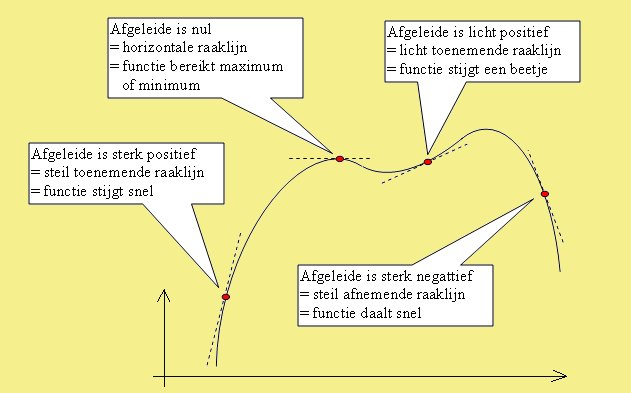
\includegraphics[width=0.8\textwidth]{afgeleide}
  \vfill
\end{center}
\vfill
\subsection*{Doelstelling}
{\singlespacing
Je \hfill  {\scriptsize(LP 2006-059, LI 1.5)}
\begin{itemize}
\item kent de definitie van afgeleid getal
\item kan bij functies met behulp van het intuïtief begrip van limiet het verband leggen tussen:
  \begin{itemize}
  \item het begrip afgeleide,
  \item het begrip differentiequotiënt,
  \item de richtingscoëfficiënt van de raaklijn aan de grafiek,
  \item de maat voor de ogenblikkelijke verandering
  \end{itemize}
\item kent het begrip afgeleide functie
\item kan de afgeleide functie bereken van $f(x)=c (c\in\mathbb{R})$, $f(x)=x$, $f(x)=x^2$, $f(x)=x^3$ en $f(x)=x^n (n\in\mathbb{N})$.
\item kan op de bovenstaande functies de somregel, de veelvoudregel, de productregel en de quotiëntregel toepassen
\item kan het verband tussen het tekenverloop van de eerste afgeleide en het opsporen van extrema en kan het verloop van een veeltermfunctie van de derde graad uitleggen
\item kan extremumvraagstukken (ook van buiten de wiskunde) die aanleiding geven tot veeltermfuncties en rationale functies, oplossen
\end{itemize}
}

\thispagestyle{empty}
\newpage
\tableofcontents
\thispagestyle{empty}
\newpage

\clearpage
\pagenumbering{arabic}

\fancyhead[RO,LE]{Afgeleiden}
\fancyhead[RE,LO]{}

\section{Differentiequotiënt}

\begin{definitie}
  We noemen het quotiënt
  $$\dfrac{f(x)-f(a)}{x-a}$$
  het {\bf differentiequotiënt in het interval $[a, x]$}.
\end{definitie}

\begin{center}
  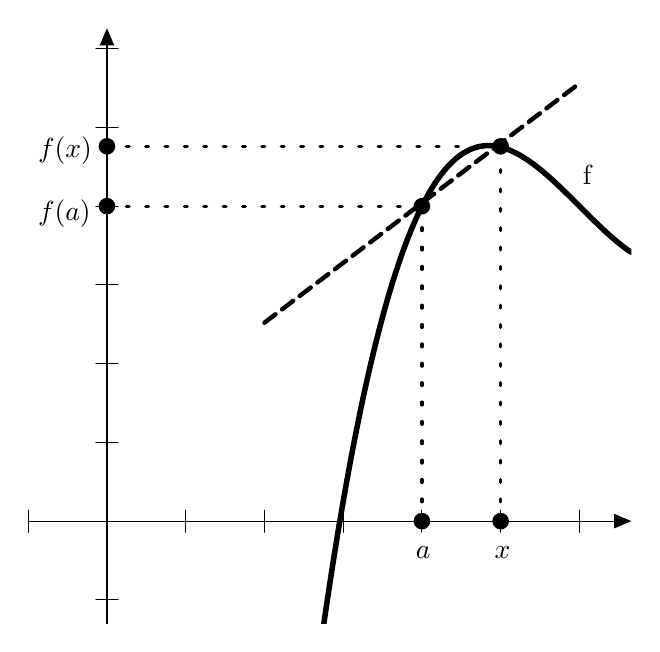
\begin{tikzpicture}[scale=2, line cap=round,line join=round,>=triangle 45,x=1.0cm,y=1.0cm]
    \draw[->,color=black] (-0.5,0) -- (3.33,0);
    \foreach \x in {-0.5,0.5,1,1.5,2,2.5,3}
    \draw[shift={(\x,0)},color=black] (0pt,2pt) -- (0pt,-2pt);
    \draw[->,color=black] (0,-0.65) -- (0,3.13);
    \foreach \y in {-0.5,0.5,1,1.5,2,2.5,3}
    \draw[shift={(0,\y)},color=black] (2pt,0pt) -- (-2pt,0pt);
    \clip(-0.5,-0.65) rectangle (3.33,3.13);
    \draw[line width=2pt, smooth,samples=100,domain=-0.5001340603726351:3.327196879862643] plot(\x,{((\x)-3)^3-(\x)+5});
    \draw [line width=1.2pt,dash pattern=on 1pt off 6pt] (0,2)-- (2,2);
    \draw [line width=1.2pt,dash pattern=on 1pt off 6pt] (0,2.38)-- (2.5,2.38);
    \draw [line width=1.2pt,dash pattern=on 1pt off 6pt] (2,0)-- (2,2);
    \draw [line width=1.2pt,dash pattern=on 1pt off 6pt] (2.5,0)-- (2.5,2.38);
    \draw [line width=1.6pt,dash pattern=on 5pt off 3pt,domain=1:3] plot(\x,{(--0.25--0.38*\x)/0.5});
    \draw (1.9,-0.1) node[anchor=north west] {$a$};
    \draw (2.4,-0.1) node[anchor=north west] {$x$};
    \draw (-0.5,2.1) node[anchor=north west] {$f(a)$};
    \draw (-0.5,2.5) node[anchor=north west] {$f(x)$};
    \draw (2.96,2.32) node[anchor=north west] {f};
    \begin{scriptsize}
      \fill [color=black] (2,0) circle (1.5pt);
      \fill [color=black] (2.5,0) circle (1.5pt);
      \fill [color=black] (2,2) circle (1.5pt);
      \fill [color=black] (2.5,2.38) circle (1.5pt);
      \fill [color=black] (0,2.38) circle (1.5pt);
      \fill [color=black] (0,2) circle (1.5pt);
    \end{scriptsize}
  \end{tikzpicture}
\end{center}

Het differentiequotiënt geeft de helling van het lijnstuk dat door de punten $(a,f(a))$ en $(x,f(x))$ loopt, zie op bovenstaande figuur.

Het quotiënt $\dfrac{f(a+h)-f(a)}{h}$ is dan analoog het differentiequotiënt in het interval $[a, a+h]$.

\begin{oefening}
  Maak zoals hierboven een grafiek van het differentiequotiënt in $[a, a+h]$.
\end{oefening}

Een differentiequotiënt in het interval $[a,b]$ kan symbolisch geschreven worden als $\dfrac{\Delta y}{\Delta x}_{[a,b]}$.

\begin{oefening}
  Gegeven de functie
  $$f(x)=x^3-9x^2+26x-22$$
  bereken het differentiequotiënt in de intervallen $[2,2.5]$, $[2.5,3]$ en $[2,3]$. Verklaar je resultaten aan de hand van een grafiek.
\end{oefening}

\pagebreak
\section{Afgeleide waarde}

\begin{definitie}
  We noemen de {\bf afgeleide waarde van $f$ in $a$}
  $$f'(a)=\lim_{h\to 0}\dfrac{f(a+h)-f(a)}{h}$$
  als het rechterlid bestaat en een reëel getal is. We zeggen dat {\bf $f$ afleidbaar is in $a$}.
\end{definitie}

In voorgaande definitie konden we ook de volgende limiet gebruiken om afgeleide waarde te definiëren:
$$f'(a)=\lim_{x\to a}\dfrac{f(x)-f(a)}{x-a}$$

De afgeleide waarde van $f$ in $a$ wordt ook nog genoteerd als $Df(a)$ of $\dfrac{\mbox{d}f}{\mbox{d}x}(a)$. Wij zullen de notatie $f'(a)$ gebruiken. We noemen de {\em afgeleide waarde} ook nog {\em afgeleid getal} of nog korter {\em afgeleide}.

\begin{oefening}
  Toon grafisch aan dat beide definities equivalent zijn.
\end{oefening}

\begin{oefening}
  Bereken het afgeleid getal:
  \begin{enumerate}[(a)]
    \itemsep.5em
  \item $f(x)=x^2$ in $x=3$
  \item $f(x)=x^2$ in $x=-1$
  \item $f(x)=x^2+3$ in $x=-1$
  \item $f(x)=x-1$ in $x=-1.5$
    % \item $f(x)=x^2-x$ in $x=3$
  \item $f(x)=23$ in $x=-2$
  \item $f(x)=\dfrac{1}{x^2}$ in $x=0$
    % \item $f(x)=\dfrac{1}{x^2}$ in $x=-2$
    % \item $f(x)=\dfrac{x+1}{x^2+4x+4}$ in $x=-1$
  \item $f(x)=\dfrac{x^2+4x+4}{x-2}$ in $x=\frac{1}{2}$
    % \item $f(x)=\dfrac{x}{x^2-x}$ in $x=-1$
    % \item $f(x)=\sqrt{x-3}$ in $x=4$
  \end{enumerate}
\end{oefening}

\begin{oefening}
  Gegeven de functie
  $$f(x)=x^3-9x^2+26x-22\;.$$
  \begin{enumerate}[(a)]
  \item Bereken $f'(2)$, $f'(2.5)$ en $f'(3)$ Teken ook de grafiek van $f(x)$.
  \item Teken de grafiek van $f(x)$.
  \item Teken de raaklijnen aan $f$ in de punten $(2, f(2))$, $(2.5, f(2.5))$ en $(3, f(3))$.
  \item Geef het verband tussen de raaklijnen aan $f$ en de afgeleide waarden.
  \end{enumerate}
\end{oefening}

\pagebreak
\section{Afgeleide functie}

\subsection{Definitie}

\begin{definitie}
  We zeggen dat de functie $f:\mathbb{R}\to\mathbb{R}$ afleidbaar is als de afgeleide waarde $f'(a)$ bestaat in elk punt $a\in\mathbb{R}$. De {\bf afgeleide functie $f'$} van $f$ is dan de functie die in elk punt $a\in\mathbb{R}$ de afgeleide $f'(a)$ als functiewaarde heeft:
  $$f':\mathbb{R}\to\mathbb{R}:x\mapsto f'(x)\;.$$
\end{definitie}

Deze afgeleide functie wordt ook nog genoteerd als $Df$ of $\dfrac{\mbox{d}f}{\mbox{d}x}$. Wij gebruiken de notatie $f'$.

\subsubsection*{Voorbeeld 1}

De functie
$$f(x)=x^2$$
is afleidbaar in $\mathbb{R}$, neem bijvoorbeeld een willekeurige $a\in\mathbb{R}$, dan geldt
\begin{align*}
  \dfrac{f(x)-f(a)}{x-a} &= \dfrac{x^2-a^2}{x-a}\\
                         &= \dfrac{(x-a)(x+a)}{x-a}\\
                         &= x+a
\end{align*}
en dus
\begin{align*}
  \lim_{x\to a}\dfrac{f(x)-f(a)}{x-a} &= \lim_{x\to a}(x+a)\\
                                      &= a+a\\
                                      &= 2a
\end{align*}
Het getal $2a$ bestaat en is reëel aangezien $a$ reëel was. De limiet bestaat en is reëel, dus wegens de definitie is $f$ afleidbaar.

\begin{oefening}
  Maak gebruik van de andere definitie voor afgeleid getal, namelijk $$f'(a)=\lim_{h\to 0}\dfrac{f(a+h)-f(a)}{h}$$ om hetzelfde aan te tonen.
\end{oefening}

\subsubsection*{Voorbeeld 2}

De functie
$$f(x)=\sqrt[3]{x}$$
is niet overal afleidbaar in $\mathbb{R}$, neem $a=0$, dan geldt
\begin{align*}
  \dfrac{f(x)-f(0)}{x-0} &= \dfrac{\sqrt[3]{x}-\sqrt[3]{0}}{x-0}\\
                         &= \dfrac{\sqrt[3]{x}}{x}\\
                         &= \dfrac{1}{\sqrt[3]{x^2}}\\
\end{align*}
en dus
\begin{align*}
  \lim_{x\to 0}\dfrac{f(x)-f(0)}{x-0} &= \lim_{x\to 0}\dfrac{1}{\sqrt[3]{x^2}}\\
                                      &= +\infty\\
\end{align*}
De limiet bestaat wel, maar is niet reëel. Wegens de definitie is de functie dus niet afleidbaar in $\mathbb{R}$.

Dit wordt wiskundig opgelost door uit het domein alle waarden te halen waar de functie niet afleidbaar is. We zeggen dan dat de functie wel afleidbaar is in een beperkt domein.

\subsection{Basisafgeleiden}

\begin{kader}
  \begin{multicols}{3}
    % \centering
    $\left(c\right)'=0$\\
    $\left(x\right)'=1$\\
    $\left(x^2\right)'=2x$\\
    $\left(x^3\right)'=3x^2$\\
    $\left(x^n\right)'=n\cdot x^{n-1}$\\
    $\left(\sqrt{x}\right)'=\dfrac{1}{2\sqrt{x}}$\\
    % $\left(e^x\right)'=e^x$\\
    % $\left(a^x\right)'=a^x\cdot\ln a$\\
    % $\left(\ln x\right)'=\dfrac{1}{x}$\\
    % $\left(\log_a{x}\right)'=\dfrac{1}{x\cdot \ln a}$\\
    % $\left(\sin x\right)'=\cos x$\\
    % $\left(\cos x\right)'=-\sin x$\\
    % $\left(\tan x\right)'=\sec^2 x$\\
    % $\left(\cot x\right)'=-\csc^2 x$\\
    % $\left(\arcsin x\right)'=\dfrac{1}{\sqrt{1-x^2}}$\\
    % $\left(\arccos x\right)'=-\dfrac{1}{\sqrt{1-x^2}}$\\
    % $\left(\arctan x\right)'=\dfrac{1}{1+x^2}$\\
  \end{multicols}
\end{kader}

\begin{oefening}
  Voorbeeld 1 hierboven gaf ons de afleiding van $f(x)=x^2$. Toon op dezelfde manier aan dat
  \begin{enumerate}[(a)]
    \itemsep.5em
  \item als $f(x)=c$ met $c \in \mathbb{R}$ dat dan $f'(x)=0$
  \item als $f(x)=x$ dat dan $f'(x)=1$
  \item als $f(x)=x^3$ dat dan $f'(x)=3x^2$
  \item* als $f(x)=x^n$ met $n\in \mathbb{R}$ dat dan $f'(x)=nx^{n-1}$
\end{enumerate}
\end{oefening}

\begin{oefening}
Gebruik de lijst met basisafgeleiden om volgende functies af te leiden:
\begin{enumerate}[(a)]
  \itemsep.5em
  \item $f(x)=x$
  \item $f(x)=x^5$
  \item $f(x)=\sqrt{x}$
  \item $f(x)=10^{100}$
\end{enumerate}
\end{oefening}

\begin{oefening}
Bepaal de afgeleide waarde van
\begin{enumerate}[(a)]
  \itemsep.5em
  \item $f(x)=x^4$ in $x=-1$, $x=1$ en $x=9$
  \item $f(x)=\sqrt{x}$ in $x=-9$, $x=0$, $x=1$ en $x=4$
  \item $f(x)=42$ in $x=10^{100}$, $x=\pi$ en $x=\sqrt{3}$
\end{enumerate}
\end{oefening}

\subsection{Eigenschappen van afgeleiden}

\begin{kader}
  \begin{itemize}
  \item {\bf somregel}
    $$(f+g)'(x)=f'(x)+g'(x)$$
    De afgeleide van een som is dus de som van de afgeleiden.
  \item {\bf veelvoudregel}
    $$(c\cdot f)'(x) = c\cdot f'(x)$$
    Een constante factor mag voorop gebracht worden.
  \item {\bf productregel}
    $$(f\cdot g)'(x)=f'(x)\cdot g(x) + f(x)\cdot g'(x)$$
    De afgeleide van een product is de afgeleide van de eerste factor maal de tweede factor plus de eerste factor maal de afgeleide van de tweede factor
  \item {\bf quotiëntregel}
    $$\left(\dfrac{f}{g}\right)'(x)=\dfrac{f'(x)\cdot g(x)-f(a)\cdot g'(x)}{g^2(x)}$$
    De afgeleide van een quotiënt is net zoals de productregel maar we vervangen de plus door een min en we delen alles door het kwadraat van de noemer.
  \item {\bf kettingregel}
    $$\left(g\left(f\left(x\right)\right)\right)'=g'(f(x))\cdot f'(x)$$
  \end{itemize}
\end{kader}

\subsubsection*{Voorbeeld van de kettingregel}

Als de functie die we moeten afleiden $(3x^2+x)^3$ is, dan kunnen we dit beschouwen als de samenstelling $g(f(x))$ met $f(x)=3x^2+x$ en met $g(x)=x^3$. We bepalen de afgeleiden:
$$f'(x)=6x+1 \qquad en \qquad g'(x)=3x^2\;.$$
Uit de kettingregel volgt dan
\begin{align*}
  \left((3x^2+x)^3\right)' & =\left(g\left(f\left(x\right)\right)\right)' =g'(f(x)) f'(x) &&\mbox{kettingregel}\\
                           & =3(f(x))^2 (6x+1) &&\mbox{vervangen $f'$ en $g'$}\\
                           & = 3(3x^2+x)^2(6x+1) &&\mbox{vervangen $f$}\\
                           & = 162x^5 + 135x^4 + 36x^3 + 3x^2 &&\mbox{uitwerken}
\end{align*}

\begin{oefening}
  Toon aan dat we met behulp van de kettingregel ook nog volgende eigenschap krijgen:
  \begin{mdframed}
    \begin{itemize}
    \item {\bf machtregel}
      $$(f^n)'(x)=n\cdot f^{n-1} \cdot f'(x)$$
    \end{itemize}
  \end{mdframed}
\end{oefening}

\begin{oefening}
  Bereken volgende afgeleiden:
  \begin{multicols}{2}
    \begin{enumerate}[(a)]
      \itemsep1em
    \item $\left(21\right)'$
    \item $\left(4x\right)'$
    \item $\left(\dfrac{1}{3}x^3\right)'$
    \item $\left(2\sqrt{x}\right)'$
    \item $\left(\dfrac{x}{\sqrt{x}}\right)'$
    \item $\left(x^2-x\right)'$
    \item $\left(x-13\right)'$
    \item $\left(3x^3+2x^2+x+1\right)'$
    \item $\left(\frac{1}{3}x^3+\dfrac{1}{2}x^2+x+1\right)'$
    \item $\left(x^4-x^3+x^2-x+1\right)'$
    \item $\left(34+23-x^{43}\right)'$
    \end{enumerate}
  \end{multicols}
\end{oefening}

\begin{oefening}
  Bereken $f'(x)$
  \begin{multicols}{2}
    \begin{enumerate}[(a)]
      \itemsep.5em
    \item $f(x)=x^3-\dfrac{1}{2}x^2-x+1$
    \item $f(x)=\left(x-3\right)^2$
    \item $f(x)=\left(2x^3-3x^2\right)^2$
    \item $f(x)=\left(2-x\right)^3$
    \item $f(x)=\left(x-2\right)\left(x+2\right)$
    \item $f(x)=\left(x-\sqrt{a}\right)\left(x+\sqrt{a}\right)$ met $a\in\mathbb{R}^+$
    \end{enumerate}
  \end{multicols}
\end{oefening}

\begin{oefening}
  Bereken volgende afgeleiden:
  \begin{multicols}{2}
  \begin{enumerate}[(a)]
  \itemsep1em
  \item $D\left((x-3x^2)(x^2+2x)\right)$
  \item $D\left[(x^7+x^5+x^3+x)(6x^6+4x^4+2x^2)\right]$
  \item $D\left[\dfrac{2}{x+x^2+x^3}\right]$
  \item $D\left[-\dfrac{3x-2x^2}{2x^2-3x}\right]$
  \item $D\left[(3x^3+1)(2x^2+1)(x+1)\right]$
  \item $D\left[(3x^2+x^6)\dfrac{x^7+3x}{x+1}\right]$
  \end{enumerate}
  \end{multicols}
\end{oefening}

\subsection{Hogere afgeleiden}

Als de afgeleide functie van een functie $f$ opnieuw afleidbaar is, dan kan $f$ een tweede maal afgeleid worden. We noteren dan de {\bf tweede afgeleide} als
$$f''(x), f^{(2)}(x), D^2f(x), \mbox{ of } \dfrac{d^2f}{dx^2}(x)$$

Analoog kunnen we afgeleide van orde drie, vier, enz. definiëren.

\begin{oefening}
  Bereken:
  \begin{multicols}{2}
  \begin{enumerate}[(a)]
  \itemsep1em
  \item $f'' \mbox{ als } f(x)=\dfrac{1}{6}x^3+\dfrac{1}{2}x^2+x+1$
  \item $f'' \mbox{ als } f(x)=\dfrac{x^2+1}{x-1}$
  \item $f^{(3)} \mbox{ als } f(x)=x^2+x+1$
  \item $f^{(4)} \mbox{ als } f(x)=x^4-x^3+x^2-x+1$
  \item $f^{(2)} \mbox{ als } f(x)=\sqrt{x}$
  \item $f^{(2)} \mbox{ als } f(x)=(x+3)\cdot(x-8)$
  \end{enumerate}
  \end{multicols}
\end{oefening}

\begin{oefening}
Bereken
$$f^{(n)} \mbox{ als } f(x)=x^n$$
en maak hier gebruik van het feit dat we het product $n\cdot(n-1)\cdot(n-2)\cdot \cdots \cdot 3\cdot 2\cdot 1$ korter kunnen schrijven als $n!$ met behulp van faculteit. Volgend jaar zien we deze notatie in meer detail.
\end{oefening}

\subsection{Oefeningen}

\begin{oefening}
  Bereken:
  \begin{multicols}{2}
  \begin{enumerate}[(a)]
  \itemsep1em
  \item $\displaystyle\left( x^2+x \right)'$
  \item $\displaystyle\left( \dfrac{1}{4}x^4+\dfrac{1}{3}x^3+\dfrac{x^2}{2}+x+1 \right)'$
  \item $\displaystyle\left( -8x^3-12x^2-24 \right)'$
  \item $\displaystyle\left( 12+8x^2-16x \right)'$
  \item $\displaystyle\left( 7x^2+28\sqrt{x} \right)'$
  \item $\displaystyle\left( \sqrt{x}+\dfrac{1}{3}\sqrt{x} \right)'$
  \item $\displaystyle\left( 19x^2-4x-23x^2 \right)'$
  \item $\displaystyle\left( 7x^8+9x^7+6x^7 \right)'$
  \end{enumerate}
  \end{multicols}
\end{oefening}

\begin{oefening}
  Bereken:
  \begin{multicols}{2}
  \begin{enumerate}[(a)]
  \itemsep1em
  \item $\displaystyle\left( x\cdot(x^2+4x^3) \right)'$
  \item $\displaystyle\left( (3x^3+2x^2+6x+2)\cdot(6x^2+3x) \right)'$
  \item $\displaystyle\left( (x^2-1)(x^2+1) \right)'$
  \item $\displaystyle\left( (x+3)^2 \right)'$
  \item $\displaystyle\left( (x+3)^3 \right)'$
  \item $\displaystyle\left( (48+2)\cdot(23-3) \right)'$
  \end{enumerate}
  \end{multicols}
\end{oefening}

\begin{oefening}
  Bereken:
  \begin{multicols}{2}
  \begin{enumerate}[(a)]
  \itemsep1em
  \item $\displaystyle\left( \dfrac{x}{x^2+4x^3} \right)'$
  \item $\displaystyle\left( \dfrac{27x+9}{3} \right)'$
  \item $\displaystyle\left( \dfrac{x^2-4}{x+2} \right)'$
  \item $\displaystyle\left( \dfrac{27-12x^2}{2x+3} \right)'$
  \item $\displaystyle\left( \dfrac{x+1}{x-1} \right)'$
  \item $\displaystyle\left( \dfrac{8x^7+4x^5+3}{x^2+4x^4} \right)'$
  \item $\displaystyle\left( \dfrac{9x^2+4x^3}{\frac{3x^3+2}{x^8+1}} \right)'$
  \item $\displaystyle\left( (7x^3+6x^7)\cdot\dfrac{3x+9}{x-1} \right)'$
  \end{enumerate}
  \end{multicols}
\end{oefening}

\begin{oefening}
  Bereken:
  \begin{multicols}{2}
  \begin{enumerate}[(a)]
  \itemsep1em
  \item $\displaystyle\left( (x^2+1)^2 \right)'$
  \item $\displaystyle\left( (x+3)^3 \right)'$
  \item $\displaystyle\left( (\sqrt{x}+x)^2 \right)'$
  \item $\displaystyle\left( 3x+(3x+4x^2)^3 \right)'$
  \end{enumerate}
  \end{multicols}
\end{oefening}

\begin{oefening}*
  Bepaal de afgeleide functie $f'$ voor de volgende functies $f$:
  \begin{multicols}{2}
  \begin{enumerate}[(a)]
  \itemsep1em
  \item $\displaystyle f(x)=(\dfrac{1}{3}x^3-\dfrac{1}{2}x^2+8)^2$
  \item $\displaystyle f(x)=\sqrt{9x^3+4x^2+x}$
  \item $\displaystyle f(x)=\sqrt{ax+b}$ met $a,b\in\mathbb{R}$ en $a\neq 0$
  \item $\displaystyle f(x)=\sqrt{x+3}\cdot(x^2+3x)^4$
  \item $\displaystyle f(x)=\dfrac{x^3-x^2}{(2+x)^8}$
  \item $\displaystyle f(x)=\dfrac{\sqrt{4x^2-3x}}{2+x}$
  \item $\displaystyle f(x)=\sqrt{(4x^2-3x+1)^3}$
  \item $\displaystyle f(x)=\sqrt{2x+(3x+4x^2)^3}$
  \end{enumerate}
  \end{multicols}
\end{oefening}

\begin{oefening}** % Bron: USolv-it: info: Afgeleide, auteur: Lie Lam, Mario Ausseloos, id: 2481
De afgeleide functie van de functie
$$f:\mathbb{R}\to\mathbb{R^+}:x\mapsto |x|$$
wordt gegeven door
\begin{enumerate}[(A)]
  \itemsep.5em
\item $f':\mathbb{R}\to\mathbb{R}:x\mapsto 1$.
\item $f':\mathbb{R}_0\to\mathbb{R}:x\mapsto 1$.
\item $f':\mathbb{R}\to\mathbb{R}:x\mapsto \begin{cases}1  & x\geq0,\\-1 & x<0\end{cases}$.
\item $f':\mathbb{R}_0\to\mathbb{R}:x\mapsto \dfrac{x}{|x|}$.
\item $f':\mathbb{R}\to\mathbb{R}:x\mapsto \begin{cases}1  & x>0,\\0  & x=0,\\-1 & x<0\end{cases}$.
\end{enumerate}
\end{oefening}

\begin{oefening} % Bron: USolv-it: Info: Rekenregels afgeleide, auteur: Kathleen Hoornaert, id: 2038
Zij $\displaystyle f(x)=\dfrac{\sqrt{x}}{x^2+3x}$. Dan is $f'(x)$ gelijk aan
\begin{enumerate}[(A)]
  \itemsep1em
  \item $\displaystyle \dfrac{-3\sqrt{x}(x+1)}{2(x^2+3x)^2}$.
  \item $\displaystyle \dfrac{x^2-2\sqrt{x}x+3x+1}{2\sqrt{x}(x^2+3x)^2}$.
  \item $\displaystyle \dfrac{x^2+x+3}{2(x^2+3x)^2}$.
  \item $\displaystyle \dfrac{x^2-x-6}{2(x^2+3x)^2}$.
\end{enumerate}
\end{oefening}

\pagebreak
\section{Functieonderzoek}



Het bespreken van het verloop van een functie $f$ kan het best aan de hand van haar afgeleide functie $f'$ als deze bestaat.

\subsection{Stijgen en dalen van een functie}

\begin{eigenschap}
  Als $f$ een reële functie is die afleidbaar is in $]a,b[$, dan geldt
  \begin{itemize}
  \item als $f'(x)>0$ voor elk punt $x$ in $]a,b[$, dan is $f$ strikt stijgend op $[a,b]$,
  \item als $f'(x)<0$ voor elk punt $x$ in $]a,b[$, dan is $f$ strikt dalend op $[a,b]$,
  \item als $f'(x)=0$ voor elk punt $x$ in $]a,b[$, dan is $f$ een constante functie op $[a,b]$.
  \end{itemize}
\end{eigenschap}

De laatste eigenschap zal meestal toegepast worden op één enkel punt, we zullen dit verder bespreken als we het over extrema hebben.

\subsubsection*{Voorbeeld}

Beschouw de grafiek van de functie $f$ (volle lijn) en van haar afgeleide $f'$ (stippellijn).
\begin{center}
  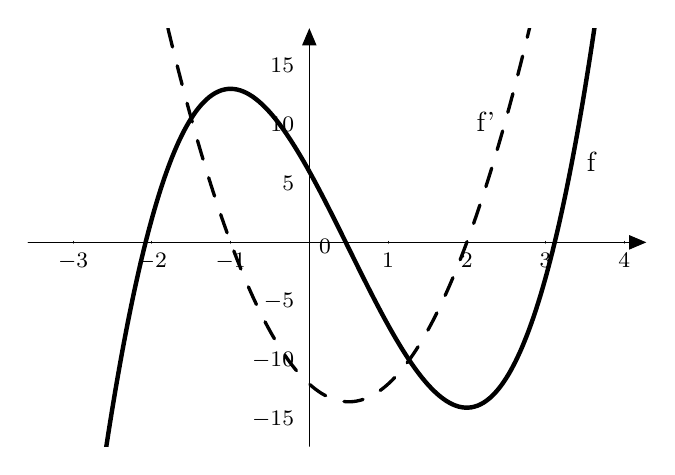
\begin{tikzpicture}[yscale=0.15, line cap=round,line join=round,>=triangle 45,x=1.0cm,y=1.0cm]
    \draw[->,color=black] (-3.57,0) -- (4.28,0);
    \foreach \x in {-3,-2,-1,1,2,3,4}
    \draw[shift={(\x,0)},color=black] (0pt,2pt) -- (0pt,-2pt) node[below] {\footnotesize $\x$};
    \draw[->,color=black] (0,-17.26) -- (0,18.13);
    \foreach \y in {-15,-10,-5,5,10,15}
    \draw[shift={(0,\y)},color=black] (-2pt,0pt) node[left] {\footnotesize $\y$};
    \draw[color=black] (0pt,-10pt) node[right] {\footnotesize $0$};
    \clip(-3.57,-17.26) rectangle (4.28,18.13);
    \draw[line width=1.6pt, smooth,samples=100,domain=-3.5716478839065284:4.279097160875563] plot(\x,{2*(\x)^3-3*(\x)^2-12*(\x)+6});
    \draw[line width=1.2pt,dash pattern=on 7pt off 7pt, smooth,samples=100,domain=-3.5716478839065284:4.279097160875563] plot(\x,{6*(\x)^2-6*(\x)-12});
    \draw (3.4,8.48) node[anchor=north west] {f};
    \draw (2,11.87) node[anchor=north west] {f'};
  \end{tikzpicture}
\end{center}
De afgeleide functie $f'$ is positief in het interval $]-\infty, -1[$. We zien aan de grafiek dat de functie $f$ in dit interval inderdaad aan het stijgen is (conform de eigenschap). In het interval $]-1, 2[$ is de afgeleide functie $f'$ negatief en de functie $f$ is daalt daar. Bepaal zelf verder het verloop van $f$ aan de hand van $f'$.

In de praktijk maken we het tekenverloop van de afgeleide functie $f'$, hierop duiden we dan het stijgen en dalen van de functie $f$ aan. In ons voorbeeld wordt dit dan:
\begin{center}
  \begin{tabular}{c|ccccc}
    $x$ & \hspace*{1.0cm} & $-1$ & \hspace*{1.0cm} & $2$ & \hspace*{1.0cm}\\
    \hline
    $f'(x)$ & + & 0 & - & 0 & +\\
    \hline
    $f(x)$ & $\nearrow$ & & $\searrow$ & & $\nearrow$
  \end{tabular}
\end{center}



\begin{oefening}
  Zoek een functie $f$, waarvoor geld $f'(x)=1\quad \forall x\in\mathbb{R}$. Maak de grafiek van $f$ en van $f'$ en maak ook het tekenverloop van $f'$ met het stijgen en dalen van $f$.
\end{oefening}

% \begin{oefening}
%   Zoek een functie $f$, waarvoor geld $f(x)=0\quad \forall x\in\mathbb{R}$. Maak de grafiek van $f$ en van $f'$ en maak ook het tekenverloop van $f'$ met het stijgen en dalen van $f$.
% \end{oefening}



\subsection{Extrema van een functie}

\begin{eigenschap}
  Als $f$ een relatief extremum heeft in $a$, dan geldt $f'(a)=0$.
\end{eigenschap}

De voorwaarde $f'(a)=0$ is niet voldoende om een relatief extremum te vinden in $a$. We kunnen hoogstens zeggen:

\begin{kader}
  Als $f'(x)=0$ in een punt $x$, dan heeft de functie $f$ {\em misschien} een extremum in $x$.
\end{kader}
Tekenonderzoek van $f'$ kan ons echter wel helpen om de extrema te vinden, we baseren ons op de volgende eigenschappen:

\begin{eigenschap}
  Als $f$ afleidbaar is in een interval rond $a$, dan geldt:
  \begin{itemize}
  \item als $f'$ overgaat van strikt negatief naar strikt positief in $a$, dan heeft $f$ in $a$ een relatief minimum,
  \item als $f'$ overgaat van strikt positief naar strikt negatief in $a$, dan heeft $f$ in $a$ een relatief maximum.
  \end{itemize}
\end{eigenschap}

In de praktijk lees je de extrema af op het tekenverloop waar $f'(x)=0$ is, zoals in ons vorig voorbeeld:

\begin{center}
  \begin{tabular}{c|ccccc}
    $x$ & \hspace*{1.0cm} & $-1$ & \hspace*{1.0cm} & $2$ & \hspace*{1.0cm}\\
    \hline
    $f'(x)$ & + & 0 & - & 0 & +\\
    \hline
    $f(x)$ & $\nearrow$ &  $\underset{=13}{\bf max}$ & $\searrow$ & $\underset{=-12}{\bf min}$ & $\nearrow$
  \end{tabular}
\end{center}

\subsection{Schetsen van een functie}

Met de kennis die we nu hebben kunnen we een strategie ontwikkelen om een functie $f$ te schetsen. Hou steeds in gedachte dat de afgeleide $f'$ enkel dient om informatie over de oorspronkelijke functie $f$ te zoeken. Het hoofddoel is niet de afgeleide, maar de functie zelf!

We gaan als volgt te werk voor een gegeven functie $f(x)=y$:
\begin{enumerate}
\item Bepaal het {\bf domein} van $f$.
\item Bepaal de {\bf nulpunten} van $f$ en duid ze aan in een orthonormaal assenstelsel.
\item Maak een {\bf tekenonderzoek} van $f$.
\item Bepaal de horizontale, schuine en verticale {\bf asymptoten} van $f$ en teken deze op de grafiek.
\item Bepaal de afgeleide functie $f'$, maak een tekenonderzoek van de afgeleide functie $f'$ en bepaal de intervallen waarop de functie $f$ {\bf stijgt of daalt}. Bepaal ook de extrema.
\item Schets de {\bf grafiek} van $f$.
\end{enumerate}

\subsection{Oefeningen}

\begin{oefening}
  Bespreek volgende functies:
  \begin{multicols}{3}
  \begin{enumerate}[(a)]
  \itemsep1em
  \item $f(x)=x^3-6x^2+11x-6$
  \item $f(x)=x^2-8x+15$
  \item $f(x)=3x^4-16x^3+24x^2$
  \item $f(x)=\dfrac{3x^2-6}{x^2+x-6}$
  \item $f(x)=\dfrac{-2x^2+7x-3}{x^2-9}$
  \item $f(x)=\dfrac{x^2-3}{2x-4}$
  \item $f(x)=\dfrac{x^3-1}{x^2}$
  \item $f(x)=\dfrac{4+3x}{x-4}-1$
  \item $f(x)=\dfrac{-3x^2-2x-4}{x^2-1}$
  \item $f(x)=\dfrac{9x^2-25}{x^3-x}$
  \end{enumerate}
  \end{multicols}
\end{oefening}

\begin{oefening}
Gegeven de grafiek van de functie $f(x)$
\begin{center}
\definecolor{cqcqcq}{rgb}{0.75,0.75,0.75}
\begin{tikzpicture}[scale=0.8,line cap=round,line join=round,>=triangle 45,x=1.0cm,y=1.0cm]
\draw [color=cqcqcq,dash pattern=on 2pt off 2pt, xstep=1.0cm,ystep=1.0cm] (-9.46,-5.51) grid (7.5,3.36);
\draw[->,color=black] (-9.46,0) -- (7.5,0);
\foreach \x in {-9,-8,-7,-6,-5,-4,-3,-2,-1,1,2,3,4,5,6,7}
\draw[shift={(\x,0)},color=black] (0pt,2pt) -- (0pt,-2pt) node[below] {\footnotesize $\x$};
\draw[->,color=black] (0,-5.51) -- (0,3.36);
\foreach \y in {-5,-4,-3,-2,-1,1,2,3}
\draw[shift={(0,\y)},color=black] (2pt,0pt) -- (-2pt,0pt) node[left] {\footnotesize $\y$};
\draw[color=black] (0pt,-10pt) node[right] {\footnotesize $0$};
\clip(-9.46,-5.51) rectangle (7.5,3.36);
\draw[line width=1.6pt, smooth,samples=100,domain=-9.459065715956372:7.503140032986307] plot(\x,{1/100*((\x)-5)*((\x)-1)*((\x)+3)*((\x)+8)});
\draw (-7.97,2.23) node[anchor=north west] {f};
\end{tikzpicture}
\end{center}
schets de grafiek van de afgeleide functie $f'(x)$.
\end{oefening}

\begin{oefening}
Gegeven de grafiek van de afgeleide functie $f'$
\begin{center}
  \definecolor{cqcqcq}{rgb}{0.75,0.75,0.75}
  \begin{tikzpicture}[scale=0.6,line cap=round,line join=round,>=triangle 45,x=1.0cm,y=1.0cm]
  \draw [color=cqcqcq,dash pattern=on 1pt off 1pt, xstep=1.0cm,ystep=1.0cm] (-5.1,-5.12) grid (5.11,5.11);
  \draw[->,color=black] (-5.1,0) -- (5.11,0);
  \foreach \x in {-5,-4,-3,-2,-1,1,2,3,4,5}
  \draw[shift={(\x,0)},color=black] (0pt,2pt) -- (0pt,-2pt) node[below] {\footnotesize $\x$};
  \draw[->,color=black] (0,-5.12) -- (0,5.11);
  \foreach \y in {-5,-4,-3,-2,-1,1,2,3,4,5}
  \draw[shift={(0,\y)},color=black] (2pt,0pt) -- (-2pt,0pt) node[left] {\footnotesize $\y$};
  \draw[color=black] (0pt,-10pt) node[right] {\footnotesize $0$};
  \clip(-5.1,-5.12) rectangle (5.11,5.11);
  \draw[line width=1.6pt, smooth,samples=100,domain=-5.099666282866462:5.106622595766759] plot(\x,{((\x)-1)*((\x)+2)});
  \draw (-3.19,1.81) node[anchor=north west] {f};
  \begin{scriptsize}
  \draw[color=black] (-3.07,5.05) node {$f$};
  \end{scriptsize}
  \end{tikzpicture}
\end{center}
bepaal de grafiek van de functie $f$:
\begin{multicols}{2}
  \begin{enumerate}[(A)]
    \item
    \begin{center}
    \definecolor{cqcqcq}{rgb}{0.75,0.75,0.75}
    \begin{tikzpicture}[scale=0.6,line cap=round,line join=round,>=triangle 45,x=1.0cm,y=1.0cm]
    \draw [color=cqcqcq,dash pattern=on 1pt off 1pt, xstep=1.0cm,ystep=1.0cm] (-5.1,-5.12) grid (5.11,5.11);
    \draw[->,color=black] (-5.1,0) -- (5.11,0);
    \foreach \x in {-5,-4,-3,-2,-1,1,2,3,4,5}
    \draw[shift={(\x,0)},color=black] (0pt,2pt) -- (0pt,-2pt) node[below] {\footnotesize $\x$};
    \draw[->,color=black] (0,-5.12) -- (0,5.11);
    \foreach \y in {-5,-4,-3,-2,-1,1,2,3,4,5}
    \draw[shift={(0,\y)},color=black] (2pt,0pt) -- (-2pt,0pt) node[left] {\footnotesize $\y$};
    \draw[color=black] (0pt,-10pt) node[right] {\footnotesize $0$};
    \clip(-5.1,-5.12) rectangle (5.11,5.11);
    \draw[line width=1.6pt, smooth,samples=100,domain=-5.099666282866462:5.106622595766759] plot(\x,{1/6*(-12*(\x)+3*(\x)^2+2*(\x)^3)});
    \draw (-3.19,1.81) node[anchor=north west] {f};
    \begin{scriptsize}
    \draw[color=black] (-3.9,-5.75) node {$f$};
    \end{scriptsize}
    \end{tikzpicture}
    \end{center}
    \item
    \begin{center}
    \definecolor{cqcqcq}{rgb}{0.75,0.75,0.75}
    \begin{tikzpicture}[scale=0.6,line cap=round,line join=round,>=triangle 45,x=1.0cm,y=1.0cm]
    \draw [color=cqcqcq,dash pattern=on 1pt off 1pt, xstep=1.0cm,ystep=1.0cm] (-5.1,-5.12) grid (5.11,5.11);
    \draw[->,color=black] (-5.1,0) -- (5.11,0);
    \foreach \x in {-5,-4,-3,-2,-1,1,2,3,4,5}
    \draw[shift={(\x,0)},color=black] (0pt,2pt) -- (0pt,-2pt) node[below] {\footnotesize $\x$};
    \draw[->,color=black] (0,-5.12) -- (0,5.11);
    \foreach \y in {-5,-4,-3,-2,-1,1,2,3,4,5}
    \draw[shift={(0,\y)},color=black] (2pt,0pt) -- (-2pt,0pt) node[left] {\footnotesize $\y$};
    \draw[color=black] (0pt,-10pt) node[right] {\footnotesize $0$};
    \clip(-5.1,-5.12) rectangle (5.11,5.11);
    \draw[line width=1.6pt, smooth,samples=100,domain=-5.099666282866462:5.106622595766759] plot(\x,{-1/6*(-12*(\x)+3*(\x)^2+2*(\x)^3)});
    \draw (-3.19,1.81) node[anchor=north west] {f};
    \begin{scriptsize}
    \draw[color=black] (-3.9,-5.75) node {$f$};
    \end{scriptsize}
    \end{tikzpicture}
    \end{center}
    \item
    \begin{center}
    \definecolor{cqcqcq}{rgb}{0.75,0.75,0.75}
    \begin{tikzpicture}[scale=0.6,line cap=round,line join=round,>=triangle 45,x=1.0cm,y=1.0cm]
    \draw [color=cqcqcq,dash pattern=on 1pt off 1pt, xstep=1.0cm,ystep=1.0cm] (-5.1,-5.12) grid (5.11,5.11);
    \draw[->,color=black] (-5.1,0) -- (5.11,0);
    \foreach \x in {-5,-4,-3,-2,-1,1,2,3,4,5}
    \draw[shift={(\x,0)},color=black] (0pt,2pt) -- (0pt,-2pt) node[below] {\footnotesize $\x$};
    \draw[->,color=black] (0,-5.12) -- (0,5.11);
    \foreach \y in {-5,-4,-3,-2,-1,1,2,3,4,5}
    \draw[shift={(0,\y)},color=black] (2pt,0pt) -- (-2pt,0pt) node[left] {\footnotesize $\y$};
    \draw[color=black] (0pt,-10pt) node[right] {\footnotesize $0$};
    \clip(-5.1,-5.12) rectangle (5.11,5.11);
    \draw[line width=1.6pt, smooth,samples=100,domain=-5.099666282866462:5.106622595766759] plot(\x,{1/6*(-12*(-\x)+3*(-\x)^2+2*(-\x)^3)});
    \draw (-3.19,1.81) node[anchor=north west] {f};
    \begin{scriptsize}
    \draw[color=black] (-3.9,-5.75) node {$f$};
    \end{scriptsize}
    \end{tikzpicture}
    \end{center}
    \item
    \begin{center}
    \definecolor{cqcqcq}{rgb}{0.75,0.75,0.75}
    \begin{tikzpicture}[scale=0.6,line cap=round,line join=round,>=triangle 45,x=1.0cm,y=1.0cm]
    \draw [color=cqcqcq,dash pattern=on 1pt off 1pt, xstep=1.0cm,ystep=1.0cm] (-5.1,-5.12) grid (5.11,5.11);
    \draw[->,color=black] (-5.1,0) -- (5.11,0);
    \foreach \x in {-5,-4,-3,-2,-1,1,2,3,4,5}
    \draw[shift={(\x,0)},color=black] (0pt,2pt) -- (0pt,-2pt) node[below] {\footnotesize $\x$};
    \draw[->,color=black] (0,-5.12) -- (0,5.11);
    \foreach \y in {-5,-4,-3,-2,-1,1,2,3,4,5}
    \draw[shift={(0,\y)},color=black] (2pt,0pt) -- (-2pt,0pt) node[left] {\footnotesize $\y$};
    \draw[color=black] (0pt,-10pt) node[right] {\footnotesize $0$};
    \clip(-5.1,-5.12) rectangle (5.11,5.11);
    \draw[line width=1.6pt, smooth,samples=100,domain=-5.099666282866462:5.106622595766759] plot(\x,{1/6*(-12*(-\x)+3*(\x)^2+2*(\x)^3)});
    \draw (-3.19,1.81) node[anchor=north west] {f};
    \begin{scriptsize}
    \draw[color=black] (-3.9,-5.75) node {$f$};
    \end{scriptsize}
    \end{tikzpicture}
    \end{center}
  \end{enumerate}
\end{multicols}
\end{oefening}

\begin{oefening}
Bepaal het tekenverloop van de afgeleide functie $f'$ als de grafiek van de functie $f$ gegeven is:
\begin{enumerate}[(a)]
  \item
  \begin{center}
    \definecolor{cqcqcq}{rgb}{0.75,0.75,0.75}
\begin{tikzpicture}[scale=0.9,line cap=round,line join=round,>=triangle 45,x=1.0cm,y=1.0cm]
\draw [color=cqcqcq,dash pattern=on 1pt off 1pt, xstep=1.0cm,ystep=1.0cm] (-5.1,-7.12) grid (5.11,3.11);
\draw[->,color=black] (-5.1,0) -- (5.11,0);
\foreach \x in {-5,-4,-3,-2,-1,1,2,3,4,5}
\draw[shift={(\x,0)},color=black] (0pt,2pt) -- (0pt,-2pt) node[below] {\footnotesize $\x$};
\draw[->,color=black] (0,-7.12) -- (0,3.11);
\foreach \y in {-7,-6,-5,-4,-3,-2,-1,1,2,3}
\draw[shift={(0,\y)},color=black] (2pt,0pt) -- (-2pt,0pt) node[left] {\footnotesize $\y$};
\draw[color=black] (0pt,-10pt) node[right] {\footnotesize $0$};
\clip(-5.1,-7.12) rectangle (5.11,3.11);
\draw[line width=1.6pt, smooth,samples=100,domain=-5.099666282866462:5.106622595766759] plot(\x,{(-90*(\x)-48*(\x)^2+2*(\x)^3+3*(\x)^4)/72});
\draw (-3.18,1.87) node[anchor=north west] {f};
\begin{scriptsize}
\draw[color=black] (-4.41,7.66) node {$f$};
\end{scriptsize}
\end{tikzpicture}
  \end{center}
  \item
  \begin{center}
    \definecolor{cqcqcq}{rgb}{0.75,0.75,0.75}
\begin{tikzpicture}[scale=0.9,line cap=round,line join=round,>=triangle 45,x=1.0cm,y=1.0cm]
\draw [color=cqcqcq,dash pattern=on 1pt off 1pt, xstep=1.0cm,ystep=1.0cm] (-3.1,-6.12) grid (7.11,4.11);
\draw[->,color=black] (-3.1,0) -- (7.11,0);
\foreach \x in {-3,-2,-1,1,2,3,4,5,6,7}
\draw[shift={(\x,0)},color=black] (0pt,2pt) -- (0pt,-2pt) node[below] {\footnotesize $\x$};
\draw[->,color=black] (0,-6.12) -- (0,4.11);
\foreach \y in {-6,-5,-4,-3,-2,-1,1,2,3,4}
\draw[shift={(0,\y)},color=black] (2pt,0pt) -- (-2pt,0pt) node[left] {\footnotesize $\y$};
\draw[color=black] (0pt,-10pt) node[right] {\footnotesize $0$};
\clip(-3.1,-6.12) rectangle (7.11,4.11);
\draw[line width=1.6pt, smooth,samples=100,domain=-3.099666282866462:7.106622595766759] plot(\x,{(48*(\x)-6*(\x)^2-16*(\x)^3+3*(\x)^4)/36});
\draw (4.78,1) node[anchor=north west] {f};
\begin{scriptsize}
\draw[color=black] (-2.44,7.66) node {$f$};
\end{scriptsize}
\end{tikzpicture}
  \end{center}
\end{enumerate}
\end{oefening}

\pagebreak
\section{Toepassingen: extremumvraagstukken}

De volgende problemen zijn extremumvraagstukken. Ze zijn één van de belangrijkste toepassingen van de eerste afgeleide. Veel studenten zijn geïntimideerd door deze problemen omdat ze de tekst eerst moeten omzetten naar een wiskundige functie. Daarnaast bestaat er geen éénduidige manier om alle extremumvraagstukken op te lossen. Echter, met een beetje geduld en de nodige oefening kan je je ongerustheid minimaliseren en je succes maximaliseren.

Volgende tips kunnen alvast handig zijn:
\begin{itemize}
\item Lees elk probleem zorgvuldig. Lees elk probleem op zijn minst drie keer voordat je het probeert op te lossen. Het is heel belangrijk dat je heel goed weet wat er wordt gevraagd. Als je hier mist of te snel gaat, dan heb je geen kans om het vraagstuk correct op te lossen.
\item Voer onbekenden in. Maak een functie hiermee en kijk of je het maximum of het minimum van die functie zoekt.
\item Probeer het aantal onbekenden te verminderen naar hoogstens één onbekende.
\item Werk systematisch, hou het stramien van onbekenden/functie/afleiden/tekenverloop en stijgen\&dalen/antwoordzin aan.
\end{itemize}

\begin{oefening}
  De som van twee positieve getallen is $2004$. Bepaal die getallen zodat hun product maximaal is.
\end{oefening}

\begin{oefening}
  De som van twee positieve getallen is $|5|$. Bepaal die getallen zodat de som van hun kwadraten minimaal is.
\end{oefening}

\begin{oefening}
  Welke rechthoek met een omtrek van $100$m heeft de grootste oppervlakte? Hoeveel bedraagt deze oppervlakte?
\end{oefening}

\begin{oefening}
  De route gevolgd door een groep bergbeklimmers wordt gegeven door de veeltermfunctie
  $$h(t)=90t^2-10t^3\;.$$
  Hierbij is:
  \begin{itemize}
  \item $h=$ de hoogte in meters,
  \item $t=$ de tijd in uren,
  \item $t=0$ is het tijdstip waarop de groep begint met de bergbeklimming.
  \end{itemize}
  Na hoeveel tijd bereiken onze klimmers de top? Op welke hoogte bevinden ze zich dan?
\end{oefening}

\begin{oefening}
  Het verkopen van koelkasten binnen een bepaalde periode wordt pas lonend bij een serieuze verkoop. In het begin is er verlies. Dat verlies wordt weergegeven door de functie
  $$v(x)=-2x^3-3x^2+36x+6\;,$$
  waarbij $x$ uitgedrukt wordt in $1000$ verkochte eenheden en $v(x)$ in $10$ euro. Voor welke verkoop is het verlies maximaal?
\end{oefening}

\begin{oefening}\\
  \begin{minipage}{0.6\textwidth}
    Uit een rechthoekig stuk karton van 40 cm lang en 20 cm breed snijdt men 6 gelijke
    vierkanten weg zoals op de figuur. Met het overblijvende deel maakt men dan een
    taartdoos. Hoe groot moet de zijde van de vierkantjes zijn opdat de taartdoos een
    maximale inhoud zou hebben? Bereken dan ook die inhoud.
  \end{minipage}
  \begin{minipage}{0.4\textwidth}
    \centering
    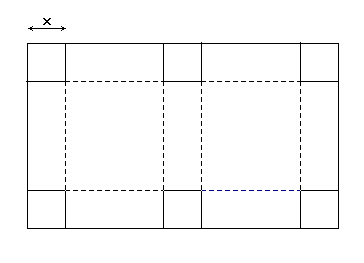
\includegraphics[width=\textwidth]{rechthoekig-stuk-karton}
  \end{minipage}
\end{oefening}

\begin{oefening}
  Oliver wil dit jaar een klein zomerfestival organiseren. Hiervoor start hij met een promotiecampagne. Een ticket kost momenteel $30$ euro. Voor elke bezoeker meer dan $250$ zal hij de ticketprijs verlagen met $0.10$ euro. Hoeveel festivalgangers (we gaan ervan uit dat er meer dan $250$ bezoekers zijn) moeten aanwezig zijn opdat de inkomsten maximaal zijn? Geef hiervoor de ticketprijs.
\end{oefening}

\begin{oefening}
  Bepaal twee getallen $x$ en $y$ waarvan de som 144 is en waarvoor het product maximaal
  is. En voor welke waarden is het product $x^3\cdot y^2$ maximaal?
\end{oefening}

\begin{oefening}
  Aan de vier hoeken van een vierkantig stuk karton met zijden van 20 cm knipt men gelijke vierkanten weg. Onderzoek het verloop van de inhoud van de doos zonder deksel die men hiermee kan vormen. Wanneer is die inhoud maximaal? Bepaal ook het maximaal volume.
\end{oefening}

\begin{oefening}\\
  \begin{minipage}{0.6\textwidth}
    Een balkvormige doos met een vierkantig grondvlak bindt men toe met een lint dat
    2 meter lang is (zoals op de figuur). Noem de zijden van het grondvlak $z$ en de hoogte
    $h$. Bepaal $z$ en $h$ waarvoor de inhoud van de doos maximaal is. Bereken dan ook die
    maximale inhoud.
  \end{minipage}
  \begin{minipage}{0.4\textwidth}
    \centering
    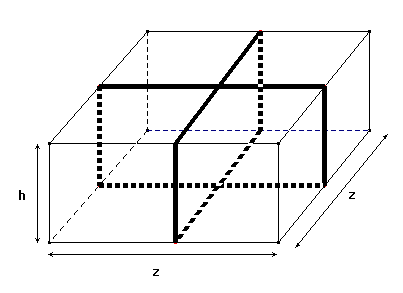
\includegraphics[width=\textwidth]{doos-met-lint}
  \end{minipage}
\end{oefening}

\begin{oefening}
  Welke rechthoek beschreven in een cirkel met straal r heeft de grootste oppervlakte?
\end{oefening}

\begin{oefening}
  Welke rechthoekige driehoek met een schuine zijde van 5 cm heeft de grootste
  oppervlakte? Bepaal dan ook de oppervlakte van deze driehoek.
\end{oefening}

\begin{oefening}
  Van een reëel getal trekken we het kwadraat af. Voor welk reëel getal is dat verschil het grootst.
\end{oefening}

\begin{oefening}
  Een frisdrankenblik heeft een inhoud van 33 cl. De oppervlakte van het stuk blik dat nodig is om het te maken hangt af van de hoogte $h$ en van de straal $r$ van het grond- en
  bovenvlak.
  \begin{enumerate}
  \item Toon aan dat $h=\dfrac{330}{\pi r^2}$
  \item Noem $A$ de totale oppervlakte van het blik. Toon aan dat $A=\dfrac{2\pi r^3 + 660}{r}$.
  \item Bepaal de afmetingen $h$ en $r$ waarvoor de totale blikoppervlakte minimaal is.
  \end{enumerate}
\end{oefening}

\begin{oefening}
  Een goudsmid vervaardigt een rechthoekig kadertje waarvan de twee overstaande zijden gouden staafjes zijn van 100 euro per cm lengte en de twee andere zilveren staafjes van 75 euro per cm lengte. Wat is de grootst mogelijke oppervlakte die hij kan bekomen als de totale kostprijs 1 500 euro mag zijn?
\end{oefening}

\begin{oefening}
  Verdeel het getal 120 in twee positieve getallen, zo dat het product van het kwadraat van het eerste getal met het tweede getal maximaal is.
\end{oefening}

\begin{oefening}
  Verdeel het getal 60 in twee positieve getallen, zo dat som van de kwadraten van de twee getallen minimaal is.
\end{oefening}

\begin{oefening}
  Een plaat van 1m breed plooi je, zo dat ze een goot vormt. Bij welke afmetingen kan door de goot een maximale hoeveelheid water stromen?
\end{oefening}

\begin{oefening}
  Uit een vierkant van 40x40cm knip je vierkantjes. Zo kan je het geheel plooien tot een doos. Hoeveel knip je weg om een zo groot mogelijke doos te bekomen?
\end{oefening}

\begin{oefening}\\
  \begin{minipage}{0.6\textwidth}
    Een ondernemer wil een rechthoekig terrein aankopen en het omheinen. Het terrein moet een oppervlakte van 1 200 m$^2$ hebben en het paalt aan een gebouw dat dus aan één zijde als afsluiting dient. De afsluiting parallel met het gebouw kost 15 euro per meter en aan de twee andere zijden 10 euro per meter. Voor welke afmetingen is de kostprijs minimaal?
  \end{minipage}
  \begin{minipage}{0.4\textwidth}
    \centering
    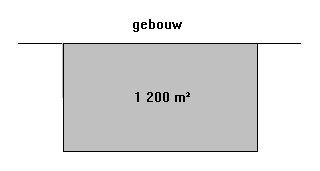
\includegraphics[width=\textwidth]{terrein-omheinen}
  \end{minipage}
\end{oefening}

\begin{oefening}
  Uit een boomstam met een diameter van 30 cm wordt een rechthoekige balk gezaagd. Het draagvermogen van zo'n balk hangt natuurlijk af van de hoogte en de breedte van de balk en is evenredig met het product $b\cdot h^2$. Bepaal de afmetingen van de balk zo dat het draagvermogen zo groot mogelijk wordt.
\end{oefening}

\begin{oefening}
  Met een draad van 1000 meter lengte omspannen we een rechthoekige weide. Bepaal de afmetingen van de weide zodat de oppervlakte zo groot mogelijk is. De draad wordt uiteraard volledig opgebruikt.
\end{oefening}

\begin{oefening}
  De totale oppervlakte van een cilindervormige doos is 12 dm$^2$. Bepaal straal en hoogte h van de doos zodat de inhoud maximaal is.
\end{oefening}

\begin{oefening}
  In een cirkel met straal 10 cm kan men verschillende rechthoeken beschrijven. Bepaal de rechthoek met de grootste oppervlakte. (tip : gebruik Pythagoras).
\end{oefening}

\begin{oefening}
  Vind de vergelijking van de rechte door het punt (3,4) die in het eerste kwadrant een
  driehoek afsnijdt met minimale oppervlakte.
\end{oefening}

\begin{oefening}
  Wat is de minimale afstand van het punt (4,2) tot de parabool $y^2 = 8x$?
\end{oefening}

% \begin{oefening}
%   In welk punt in het eerste kwadrant van de parabool $y=4-x^2$ bepaalt de raaklijn
%   samen met de coördinaatassen een driehoek met minimale oppervlakte.
% \end{oefening}

%%%%%%%%%%%%%%%%%%%%%%%%%%%%%%%%%%%%%%%%%%%%%%%%%%%%%%%%%%%%%%%%%%%%%%
\end{document}

